%%% Local Variables:
%%% mode: latex
%%% TeX-master: t
%%% End:

\documentclass[bachelor,adobefonts]{thuthesis}
%\documentclass[master]{thuthesis}
%\documentclass[doctor]{thuthesis}
% \documentclass[%
%   bachelor|master|doctor|postdoctor, % mandatory option
%   winfonts|nofonts|adobefonts, % mandatory only for bachelor and Linuxer
%   secret,
%   openany|openright,
%   arialtoc,arialtitle]{thuthesis}
% 当使用 XeLaTeX 编译时,本科生、Linux 用户需要加上 nofonts 选项;
% 当使用 PDFLaTeX 编译时,adobefonts 选项等效于 winfonts 选项(缺省选项)。

% 所有其它可能用到的包都统一放到这里了,可以根据自己的实际添加或者删除。
\usepackage{thutils}
\usepackage{amsmath}
\usepackage[ruled,vlined]{algorithm2e}
\usepackage{graphicx}
\usepackage{multirow}


\renewcommand{\algorithmcfname}{算法}
% 你可以在这里修改配置文件中的定义,导言区可以使用中文。
% \def\myname{薛瑞尼}
\theorembodyfont{\songti}
\theoremheaderfont{\heiti}

\begin{document}
% 定义所有的eps文件在 figures 子目录下
\graphicspath{{figures/}}

%%% 封面部分
\frontmatter

%%% Local Variables:
%%% mode: latex
%%% TeX-master: t
%%% End:
\secretlevel{绝密} \secretyear{2100}

\ctitle{社交数据中的活动挖掘}
% 根据自己的情况选,不用这样复杂
\makeatletter
\ifthu@bachelor\relax\else
  \ifthu@doctor
    \cdegree{工学博士}
  \else
    \ifthu@master
      \cdegree{工学硕士}
    \fi
  \fi
\fi
\makeatother

\cdepartment[计算机]{计算机科学与技术系}
\cmajor{计算机科学与技术}
\cauthor{王凝枰} 
\csupervisor{唐 杰 副教授}

% 日期自动生成,如果你要自己写就改这个cdate
%\cdate{\CJKdigits{\the\year}年\CJKnumber{\the\month}月}

% 博士后部分
% \cfirstdiscipline{计算机科学与技术}
% \cseconddiscipline{系统结构}
% \postdoctordate{2009年7月——2011年7月}

\etitle{Activity Mining in Social Media} 
% 这块比较复杂,需要分情况讨论:
% 1. 学术型硕士
%    \edegree:必须为Master of Arts或Master of Science(注意大小写)
%              “哲学、文学、历史学、法学、教育学、艺术学门类,公共管理学科
%               填写Master of Arts,其它填写Master of Science”
%    \emajor:“获得一级学科授权的学科填写一级学科名称,其它填写二级学科名称”
% 2. 专业型硕士
%    \edegree:“填写专业学位英文名称全称”
%    \emajor:“工程硕士填写工程领域,其它专业学位不填写此项”
% 3. 学术型博士
%    \edegree:Doctor of Philosophy(注意大小写)
%    \emajor:“获得一级学科授权的学科填写一级学科名称,其它填写二级学科名称”
% 4. 专业型博士
%    \edegree:“填写专业学位英文名称全称”
%    \emajor:不填写此项
\edegree{Bachelor of Engineering} 
\emajor{Computer Science and Technology} 
\eauthor{Ningping Wang} 
\esupervisor{Associate Professor Jie tang} 

% 这个日期也会自动生成,你要改么?
% \edate{December, 2005}

% 定义中英文摘要和关键字
\begin{cabstract}
随着社交媒体和移动互联网日益渗透用户的日常生活,用户越来越多的在社交媒体上发布和自己的日常生活相关的内容。社交数据中对用户日常活动信息的挖掘,可以在用户行为建模,个性化推荐等领域有着诸多潜在应用。然而,活动挖掘这个领域并没有得到足够的重视,这方面仅由很少量的工作。本文基于微博这一流行的社交网络,研究了在社交数据中进行活动挖掘的算法和框架。

本文将活动信息挖掘分解为多个子问题,首先从微博文本中抽取活动概念;其次,抽取活动相关属性,包括时间、地点、情感极性等,构成活动实例。基于概念抽取和实例抽取的结果,对活动的相关度和序列关系进行挖掘。

此外,本文构建了关于日常活动的知识库系统ActivityNet,对于用户的查询请求,通过地图、图表等形式,将上述工作得到的活动相关知识进行直观的展示。
\end{cabstract}

\ckeywords{活动挖掘,自然语言处理,信息抽取,社交媒体,知识库}

\begin{eabstract} 
As social media and mobile network gain popularity in people's everyday life, people are posting more and more activity-related content in social media. Activity mining in social data offers tons of potential applications, such as user behavior modeling and personalized recommendation. However, this area has not attracted much attention so far. Based on Weibo, one of the most popular social network in China, the thesis studies the algorithms and frameworks of activity mining in social data.

This work treats activity mining as a series of sub-problems. First, extracting abstract activity concept in social content. Then, extracting activity attributes including place, time, sentiment polarity and building activity instances. Based and concept extraction and instance extraction result, mining similarity and seqential relations between activities.

Besides, a knowledge-base system Activity is built to demonstrate our work. In response to user's query, a visualized respresention of the knowledge about the activity is shown, using maps and charts.
\end{eabstract}

\ekeywords{Activity Mining, Natural Language Processing, Information Extraction, Social Media, Knowledge Base}

% 设置 PDF 文档的作者、主题等属性
\makeatletter
\thu@setup@pdfinfo
\makeatother
\makecover

% 目录
\tableofcontents

% 符号对照表
\begin{denotation}

\item[HPC] 高性能计算 (High Performance Computing)
\

\end{denotation}



%%% 正文部分
\mainmatter
\chapter{绪论}
\section{研究背景和意义}
在过去几年中,世界见证了以Facebook,Twitter,以及国内新浪微博、人人网为代表的社交网络的崛起。Facebook全球已经有超过10亿用户,新浪微博全球注册用户已经达到6亿。据报道,在美国,人们16\%的上网时间停留在Facebook上,超过了传统搜索引擎Google的10\%。社交媒体中保存了大量的用户资料,用户间的社交关系以及海量文本信息,有着巨大的研究价值,在广告和推荐系统方面,也有着广阔的应用前景。

\begin{figure}[!h]
\centering
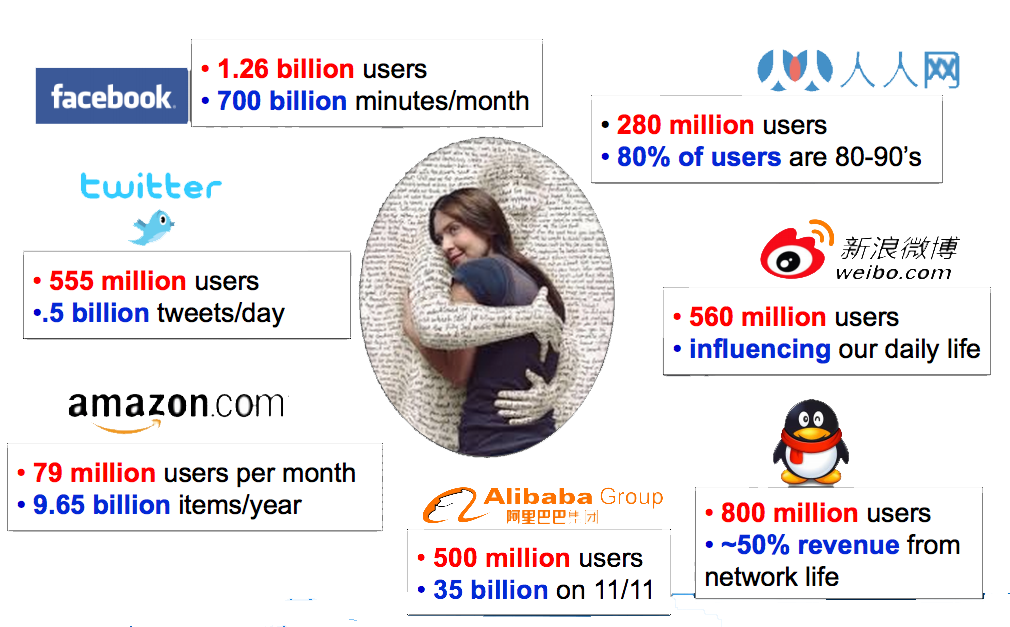
\includegraphics[width=0.8\textwidth]{social_pros.png}
\caption{社交网络的崛起}
\end{figure}

社交网络为用户提供了一个信息传播,结识好友的社交平台,用户发布的信息最初也通常是交流、沟通以及对社会事件的看法。现有的社交网络研究,如网络结构和演化分析\cite{leskovec2008microscopic}, 链接预测\cite{liben2007link}, 影响力分析\cite{tang2009social}, 社会纽带关系推断\cite{tang2011learning}等,更多地考虑社交网络本身的特性和用户的线上行为。而随着移动的互联网的迅猛发展和智能移动通信工具的普及,用户访问社交网络不再局限于传统的个人计算机。朋友聚会,家庭出游等活动中,经常许多人到达目的地的第一件事是拿出手机,在微博或Foursquare等社交网络上签到,告诉朋友们自己现在在做什么,心情如何,社交网络和线下的日常生活以前所未有的方式深入地结合在一起。这也促使我们关注这样一个问题,是否可以从社交媒体的海量数据中挖掘出人们日常活动中的一些知识,比如一项活动通常在什么时间、什么地点发生,两个活动是否存在联系,用户在进行A活动后,最可能去做的下一件事是什么。最终将我们得到的数据进行整理、分析,并实现一个可视化的系统,方便进一步的分析和应用。

相比于其他的Web数据,如点评、论坛、百科、问答平台,社交媒体有不可替代的优势。大众点评、Yelp等点评类网站,同样可以挖掘用户的活动信息,但它以商家为中心,局限于用户消费行为,如就餐、住宿、电影,收集的只是用户对于商家的点评信息。而用户的日常活动,如散步、睡觉等等,用户是不会发布在这些平台上的。用户在类似微博、人人网的社交媒体上,更愿意发布私人化、生活化的内容;同时,得益于移动互联网,用户通过随时随地方便地访问社交平台,获取信息的实时性更好,也更容易获取用户精确的地理信息。同时,社交网络的好友机制,可以帮助我们推断用户在活动中的互动。例如,用户A在时刻$t$发布了一条活动信息的微博并提到了用户B,或者B在相近的地点进行了签到,我们可以推测,B参加了A提到的那一项活动,即使B并没有特意发微博表明这一事实。

对社交网络中活动信息的挖掘,可以预想,有许多潜在的应用,尤其是在推荐系统的应用。
\begin{enumerate}
\item{\heiti 用户行为模式建模} 给定用户$t_0$时刻前的活动历史$history = \{a_t|t<t_0\}$,预测用户在下一时刻$t_0+1$在地点$p$进行活动$a$的概率,即预测$P(p_i, a_j|t+1,history)$。
\item{\heiti 基于兴趣的好友推荐} 现有的社交平台,如Facebook, 人人网等的好友推荐,主要对用户是否认识进行链接预测;而微博的推荐关注,则考虑到被推荐用户的影响力,以及和用户选定兴趣标签的匹配程度。如果我们能对用户参加活动的类别和地点有足够多的了解,就能更精确地向用户推荐兴趣相投的朋友,并且更容易转化为线下的好友关系。
\item{\heiti 个性化的活动推荐} 当用户来到一个陌生的城市,或是有闲暇的时间而不知道如何休闲娱乐,我们可以基于活动的知识,向其推荐活动。比如,一个用户经常在微博中发布吃火锅类似的信息,那么,如果用户来北京旅游,就可以向其推荐东来顺等有特色的涮肉火锅,这也会产生潜在的商业价值。
\end{enumerate}

\section{研究问题与挑战}

本文目标在于建立一个关于社交媒体中活动的系统ActivityNet,并实现以下功能

\begin{enumerate}
\item 对于用户的查询,呈现该活动的相关知识,如活动的类别,地域、时间分布,类似活动等等。
\item 对于特定的社交网络用户(本文工作主要基于新浪微博),分析其活动偏好。
\item 对于给定的地点,推荐当地最热门的活动。
\end{enumerate}

我们在两个层面上研究日常活动。其中,活动的概念是抽象意义上的活动类别,定义为
\begin{definition}[活动概念(Activity Concept)]
活动的概念$c$是表示人类日常活动的动词短语,即二元组<动作(action),目标(object)>。其中,动作为动词,目标为名词。对于某些活动,目标可以为空,以O表示。例如,以下均为合法的活动。
\label{def:instance}
\begin{itemize}
\item <吃,烤鸭>
\item <参加,会议>
\item <游泳,O>
\item <旅游,O>
\end{itemize}
\label{def:concept}
\end{definition}

而活动的实例是活动概念的具体化,包含活动的概念(类别)以及相关属性,定义为
\begin{definition}[活动实例(Activity Instance)]
活动实例为五元组$a=<c, u, s, p, t>$, 其中$c$表示活动的概念,$u$为活动的执行者,$p$为发生的地点,$s$为用户的情感倾向,$t$为发生的时间。
\end{definition}

在系统构建过程中,我们需要解决以下问题:

\begin{problem}[活动挖掘]
\begin{itemize}
\item 从社交媒体的预料中中抽取活动的抽象概念表示。
\item 对一条用户发布的信息,构建活动的实例。包括活动概念,情感、地点、时间等相关属性。
\item 建模活动之间的关系。我们希望构建一个层次结构,活动之间的关系有不同的类型,例如``A is-a B'',表示B是A概念的外延(如``吃早饭''和``吃饭'');``A follows B''表示A常在B之后依次进行。
\item 对得到的知识进行高效地存贮、检索和可视化。
\end{itemize}
\end{problem}

虽然社交媒体相比其他Web数据有诸多优势,其本身的特点也给我们的工作提出了许多挑战:

\begin{enumerate}
\item 问答、论坛等Web平台,其自身的分类系统限定了话题,人们谈论的内容比较单一。而社交媒体中,人们谈论的话题不收限制,可以对自己感兴趣的任何问题发表观点,不仅仅局限在日常活动,不可避免了噪声和稀疏性问题。同时,人们在社交媒体上发布的消息格式高度自由,长度很短,同时常带有俚语和语法、词法的错误。这对信息的精确抽取带来挑战。
\item 社交媒体中对消息长度有严格限制,传统的基于统计的方法不易应用于挖掘活动之间的概念联系。
\item 利用社交网络的结构信息,如好友关系,对未明确表达的参与关系进行推断。
\end{enumerate}

在本文中,主要解决前两个挑战。对隐式的活动参与进行推断有比较大的难度,同时也不十分迫切,在将来的工作中会进一步研究。

\section{论文组织}
本文的章节安排如图\ref{fig:organ}所示。

{\heiti 第二章} 介绍了活动挖掘的相关研究领域,如信息抽取,本体学习,知识库等。

{\heiti 第三章} 介绍了基于基于神经网络语言模型和分类算法的概念抽取模型,并对结果进行了分析。

{\heiti 第四章} 介绍了抽取活动相关属性,如情感极性、地点等,构建活动实例的方法。并基于实例抽取结果,进行活动关系挖掘。

{\heiti 第五章} 介绍了本文研究中构建的系统ActivityNet,从系统的基础架构和可视化方面对该系统进行详细的介绍。

{\heiti 第六章} 对本文的工作进行总结,并提出进一步的研究方向。

\begin{figure}[!h]
\caption{论文组织}
\label{fig:organ}
\begin{center}
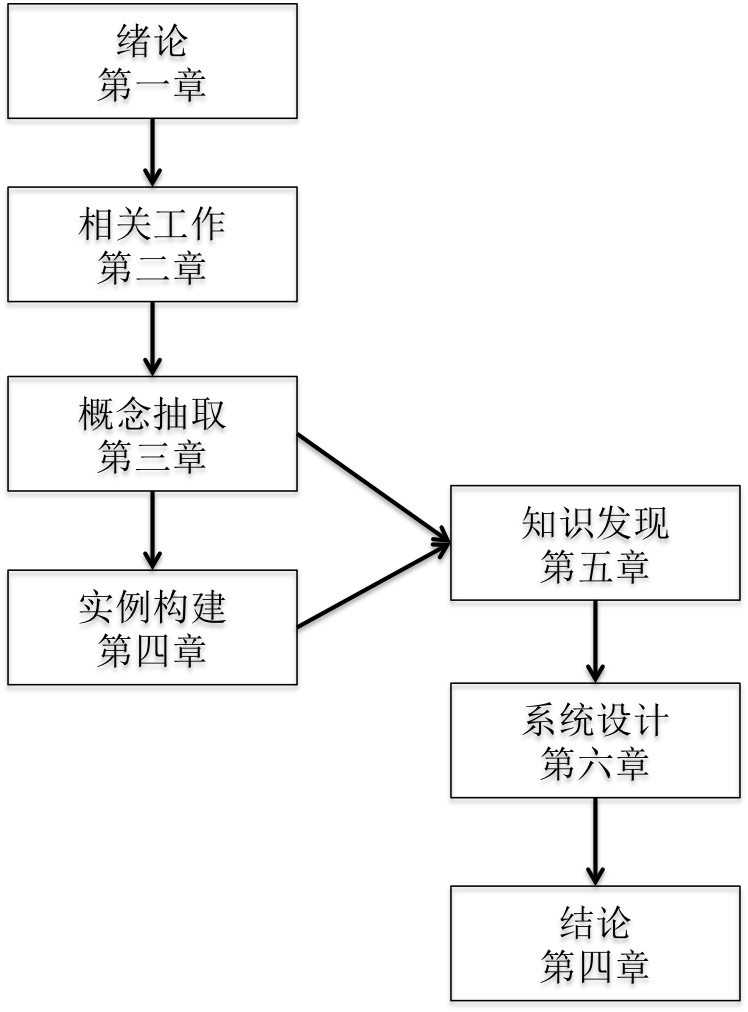
\includegraphics[width=0.5\textwidth]{organ.png}
\end{center}
\end{figure}



\chapter{相关工作}
本文实验的系统,与信息抽取、本体学习等领域有较强的相关性,同时用到了自然语言处理、机器学习的一些模型和方法。下面对本文主要的相关工作作简单的介绍。
\section{信息抽取}
信息抽取(Information Extraction)
\section{本体学习}
本体学习(Ontology Learning)

\section{知识库}
知识库是对人类知识的结构化表示,它在搜索、智能系统中有着日益重要的应用,Google,Microsoft以及国内百度、搜狗等互联网企业均有自己的知识图谱计划。下面是常见知识库概况的一个总结。

\begin{table}[!h]
\begin{tabular}[0.7\textwidth]{|l|p{2cm}|l|p{4cm}|}
\hline
名称 & 开发者 & 概念数量  & 概述 \\
\hline
SenticNet & 南洋理工大学、新加坡国立大学 & 14,244	& 情感词汇  \\
\hline
Freebase & 社区	& 1450	& 对不同领域的知名人物、地点、事物 \\
\hline
WordNet\cite{miller1995wordnet} & 普林斯顿大学 & 25,229 & 英语词汇的知识库,根据同义语将英语词汇进行组织,并且提供词汇之间的多种语义关系。 \\
\hline
WikiTaxonomy\cite{ponzetto2007deriving}	& HITS & 127,325 & 基于维基百科(Wikipedia)的语料, 将类别按照is-a关系构建为一个大规模分类系统 \\
\hline
\end{tabular}
\caption{现有知识库概况}
\label{table:knowledge_base}
\end{table}

从表\ref{table:knowledge_base}中可以看到,现有的知识库种类繁多,但主要关注词汇,客观实体如人物、地点、物体的关系建模,没有对人类日常活动给予足够的关注。希望我的工作能在这方面对现有的知识库的一个补充。

\section{情感分析Sentiment Analysis}
我们希望了解用户参与



\chapter{活动概念抽取}
\section{数据来源}
我使用了通过API抓取的新浪微博以及腾讯微博的数据。

\section{分词及词性标注}
中文分词一直自然语言处理中很基础的一步,常用的中文分词工具,如哈工大的LTP,中科院的ICTCLAS, Stanford Parser,实际应用中都难以做到非常高的准确度,尤其是在微博这种格式自由,用语不规范的文本中。综合比较各个工具的速度、精度后,我选择了ICTCLAS作为分词工具。

\section{短语抽取}
一项活动通常以一个动词(如睡觉,游泳,跑步)或者一个动词和一个名词对象组成的动宾短语(如吃午饭,去学校,打篮球)表示。为了挖掘出微博中表达的活动,我们需要将频繁出现的短语抽取出来,以待进一步处理。

最简单的方法是,遍历语料,统计所有动词短语(包括单独的动词,相邻的动词和名词)的频度,按照词频保留TopK个。这样做有两个问题
\begin{itemize}
\item 受停用词影响很大。汉语中的一些停用词,如``是'', 常被归为动词。另一些虽然不是传统意义上的停用词,一般不做为一个动作,而是副词,如``完''”,``过'' 但经常出现在动词短语中,如``做完作业'',``吃过午饭''等,干扰短语的识别。这些词的数量有限,可以简单总结,扩充已有的停用词典,预先进行过滤。
\item 目标短语在文本中可能不是连续的。除了上面举过的例子之外,动词和名词之间可能包含一些更复杂的语言成分,如``买了一件衣服'', ``参加学校举办的比赛''。由于当前的目标是抽取常见的动词短语,而并不关注单句话的精确解析,因此可以忽略过于复杂的情况,将一些常见情形总结成规则进行匹配。
\item 倾向于选取包含高频词的短语。多次同时在一起的动词、名词组合不一定是一个合法的短语,而仅仅基于词频选取短语,会倾向于包含高频词的词组。如果一个词出现次数非常高,它随机地和其他词语一起出现的次数也相应增加,导致抽取结果中包含很多噪声。为了解决这一问题,我们衡量两个词$<w_i, w_j>$构成词组概率为
$\frac{P(<w_i, w_j>)}{P(w_i)P(w_j)}$, 同时限定$n_{<w_i,w_j>} > min_support$.最后,我们按照$ln(n_{<w_i, w_j>}) + \lambda\frac{P(<w_i, w_j>)}{P(w_i)P(w_j)}$递减选取了160,000条候选短语。
\end{itemize}

\section{获取语义向量表示}

\subsection{目标与相关背景}
接下来,我们需要对得到的短语,包括unigrams和bigrams进行分类,以识别哪些短语表示一个活动。对于bigrams,它由一个动词和名词组成,一种显而易见的想法是,包含特定动词的短语,比如( 吃, ), (去, ) 更有可能是一个Activity,如果我们进行足够多的标注,就能进行有效的分类.即,每个词对应一个向量,词$w_i$对应的向量中,只有对应词序号的分量为1,即$(0_1, 0_2, ... , 1_i, ... , 0_n)$, 在计算语言学中称为One-hot Representation. 把它作为特征训练分类器.但这样做有很大的问题。直觉上,假如两个词的语义相似,那么他们的类标更有可能相同;而One-hot representation完全没有考虑词之间的语义相关性,我们能进行的标注量有限,反映到结果上就是精度尚可,但召回率非常低。我们需要找到一种有效的方式衡量两个词的语义相似性。如果能把词表示成一个K维语义空间中的一个向量,K远远小于不同词的总数,用向量的余弦相似度或者欧氏距离来衡量相似性,是最理想的,这是词的Distributed Representation,它由Hinton在1986年提出\cite{hinton1986learning}。

\subsection{话题模型}
以LDA\cite{blei2003latent}为代表的话题模型可以作为一种获得单词向量表示的方法。TODO

\subsection{n-gram 语言模型}
要对语义进行建模,容易想到的思路是,假如两个词经常出现的上下文相似,那么它们的语义可能也是相似的,这是自然语言处理中了统计语言模型的基础。一个语言模型是语言基本单位(如句子)的生成模型,用各个单词出现的条件概率来表示,即
\[
p(sentence) = \prod\limits_t {p({w_t}|Context_t)}
\]
Context的选取不同,语言模型也随之变化,其中n-gram语言模型是其中常用的一种。它对语言的生成做了n-1阶Markov假设,一个词的出现概率仅和前n-1个词相关,即
\begin{align*}
Context_t = & w_{t-n+1}^{t-1} \\
		= & (w_{t-n+1}, w_{t-n+2}, \ldots, w_{t-1}) \\
p(sentence) = & \prod\limits_t {p({w_t}|w_{t-n+1}^{t-1})}
\end{align*}

n-gram语言模型的问题是,由于语料的限制,高阶的语言模型受制于数据的稀疏性,无法建模更远的关系,一般使用tri-gram。随着互联网带来的海量数据以及计算能力的提升,更高阶的语言模型成为可能,Google曾经公开了5-gram的语言模型,但体积非常大,对我们的应用来说不切实际的。

其次,n-gram对语义相似度建模的能力有限。它仅考虑词在给定上下文出现的概率,但对上下文的相似性没有考虑。比如,``房间里趴着一只狗''和``卧室里趴着一只猫'',对``猫''和``狗''建模时,n-gram模型没有考虑``房间''和``卧室''的相似性,而它们的相似性是可以根据其他文本得到的。我们需要找到一种可以将上下文相似性一并考虑的方法模型。

\subsection{神经网络语言模型(NNLM)}
换个角度思考,我们要求的是$p({w_t}|w_{t-n+1}^{t-1})$, 实际可以看做是一个函数$f(w_{t-n+1}, w_{t-n+2}, \ldots, w_{t-1}, w_t)$. Hornik等人证明了,带有一个隐含层的多层前馈神经网络,可以近似$R^n$上任意连续函数(universal approximation theorem\cite{hornik1991approximation}). 因此,我们也能用神经网络来逼近$f()$. 我们把$w_{t-n+1}, w_{t-n+2}, \ldots, w_{t-1}$的One-hot Representation作为输入,希望输出$output_i=P(w_t=i|w_{t-n+1}, w_{t-n+2}, \ldots, w_{t-1})$, 这样就是n-gram语言模型的神经网络近似。如果我们把输入换成每个词对应的K维向量表示,那么上下文的相似性可以自然体现在向量的相似性中,这个模型就是神经网络语言模型(NNLM)\cite{bengio2006neural} \cite{mikolov2013efficient}。与一般神经网络不同的是,它的输入,即每个词的向量表示,是未知的,需要和模型参数一同优化。

\subsection{使用前馈神经网络训练NNLM}

\subsection{案例研究}
我们在1300万条新浪微博上训练了NNLM,并对得到的向量做一些案例研究,以检验模型的有效性。

通过神经网络语言模型训练得到的词向量,的确反映了语义层面上的特征,可以用余弦相似度衡量两个词语义上的相关性。我们给出一个活动,找出和其最相似的10个词组,衡量其相关性:

\begin{table}[h]
\centering
\begin{subtable}{0.3\textwidth}
     \begin{tabular}{|l|c|} 
	\hline
	{\heiti 短语} & {\heiti 相似度} \\
	\hline
	打\_篮球 & - \\
	\hline
	打球 & 0.800 \\
	\hline
	踢\_足球 & 0.790 \\
	\hline
	打\_网球 & 0.789 \\
	\hline
	打\_羽毛球 & 0.797 \\
	\hline
	踢球 & 0.727 \\
	\hline
	踢\_球 & 0.697 \\
	\hline
	练\_球 & 0.686  \\
	\hline
	游泳 & 0.667 \\
	\hline
	排球 & 0.651 \\
	\hline
	打\_排球 & 0.649 \\
	\hline
	\end{tabular}
\end{subtable}
\hspace{1em}
\begin{subtable}{0.3\textwidth}
	\begin{tabular}{|l|c|} 
	\hline
	{\heiti 短语} & {\heiti 相似度} \\
	\hline
	打扫 & - \\
	\hline
	打扫\_卫生 & 0.805 \\
	\hline
	收拾 & 0.757 \\
	\hline
	洗\_衣服 & 0.747 \\
	\hline
	家里\_打扫 & 0.699 \\
	\hline
	收拾\_屋子 & 0.693 \\
	\hline
	搞\_卫生 & 0.666 \\
	\hline
	捣鼓 & 0.659 \\
	\hline
	打扫\_打扫 & 0.659 \\
	\hline
	洗\_床单 & 0.654 \\
	\hline
	拖\_地板 & 0.652 \\
	\hline
	\end{tabular}
\end{subtable}

\begin{subtable}{0.3\textwidth}
	\begin{tabular}{|l|c|} 
	\hline
	{\heiti 短语} & {\heiti 相似度} \\
	\hline
	吃\_晚饭 & - \\
	\hline
	吃\_午饭 & 0.920 \\
	\hline
	晚饭 & 0.844 \\
	\hline
	吃\_中饭 & 0.831 \\
	\hline
	吃饭 & 0.816 \\
	\hline
	吃\_夜宵 & 0.795 \\
	\hline
	吃\_早饭 & 0.780 \\
	\hline
	午饭 & 0.777 \\
	\hline
	出去\_觅食 & 0.755 \\
	\hline
	中午\_饭 & 0.746 \\
	\hline
	喝\_早茶 & 0.736 \\
	\hline
	\end{tabular}
\end{subtable}
\hspace{1em}
\begin{subtable}{0.3\textwidth}
	\begin{tabular}{|l|c|} 
	\hline
	{\heiti 短语} & {\heiti 相似度} \\
	\hline
	下班 & - \\
	\hline
	上班 & 0.751 \\
	\hline
	回家 & 0.748 \\
	\hline
	下班\_回家 & 0.730 \\
	\hline
	坐\_班车 & 0.716 \\
	\hline
	提早\_下班 & 0.706 \\
	\hline
	回到\_家 & 0.705 \\
	\hline
	十一点\_半 & 0.705 \\
	\hline
	五点\_下班 & 0.703 \\
	\hline
	吃\_晚饭 & 0.701 \\
	\hline
	收工 & 0.698 \\
	\hline
	\end{tabular}
\end{subtable}

\caption{相似度实例}
\end{table}


并且词向量具有可加性.例如, 可以用向量加法来表达语义关系的组合:
\begin{align*}
	v(\text{济南}) - v(\text{山东}) + v(\text{浙江}) \approx & v(\text{杭州}) \\
	v(\text{北京}) - v(\text{中国}) + v(\text{法国}) \approx & v(\text{巴黎}) \\
\end{align*}
这里的约等于号表示,在所有的词中,约等号右边的词与左边运算的结果余弦相似度最大.这两个式子的含义是,杭州对浙江的关系,与济南对山东的关系相似(都是省会); 东京对日本的关系,与北京对中国的关系相似(都是首都).

再比如
\begin{align*}
	v(\text{喝}) - v(\text{渴}) + v(\text{饿}) \approx & v(\text{吃}) \\
	v(\text{校长}) - v(\text{学校}) + v(\text{公司}) \approx & v(\text{总裁}) \\
	v(\text{胡锦涛}) - v(\text{中国}) + v(\text{日本}) \approx & v(\text{首相}) \\
\end{align*}

这些式子都有很明确自然的语义关系.
当然,这种语义组合的关系并不是总能成立.

\section{最优化标注集}

下一步,我们对抽取出的候选集进行分类。每个短语可以看做K维语义向量空间中的一个向量,更确切来说,由于每个向量的模长均为1,它们分布在一个K维超球面上.并且由于语义的复杂性,正例(表示活动的短语)和负例(无关短语)是线性不可分的。对于模型的选择,我们主要考虑使用现有的可处理非线性情形的机器学习模型,如K近邻,支持向量机SVM,决策树等等,逻辑回归Logistic Regression等线性模型也进行测试。

分类器训练通常需要对训练样本进行标注,人工识别每个短语的类别,以确定模型参数,训练样本一般是从待分类数据中随机抽样得到。由于语义空间很大,待分类的数据也比较多,而我使用随机抽样得到的训练样本直接训练一个SVM分类器,精度可以达到76\%, 但是召回率非常低,只有43\%。更多的标注可以改善召回率低的情况,但是由于数据量很大,大量标注是很耗时的。由于数据分布的特殊性,我希望设计一种有原则的(Principled)训练样本抽取方法,在标注数据量一定的情况下,能够尽可能提高训练的效果。假设标注集为$L$,我们需要恰当定义其效用函数$Q(L)$以判断它的有效性,并且在一定约束条件下,找出最优的$L$,也就是

\[
    L^* = \arg\max_{L,|L| = M} Q(L)
\]

直觉上考虑,标注一个训练样本后,和此训练样本相似的样本,我们有较高的置信度将其正确分类。以K近邻分类器为例,对于每个未知样本,寻找训练集中和其距离最近的K个样本,由这K个近邻投票确定此样本的类标。但在我们的问题中,样本间的相似性$sim(v_i, v_j)$使用向量的余弦相似度来表示$<v_i, v_j$,据此可以定义一个样本$v$和集合$S$的相似性。

\begin{definition}
\[
    sim(v, S) = sim(v, u),|\{ {v_j}|sim({v_j},v) \ge sim(u,v)\} | = K
\]
\end{definition}

即,集合中和$v$第K个和其最相似的元素的相似度。设全部样例的集合为$U$, 标注集为$L$, 我们的效用函数可以定义成
\[
    Q(L) = \mathop {\min }\limits_{{v_i}} si{m_K}({v_i},L)
\]

目标是找到最优的标注集$L^*$。我们的问题可以形式定义为:
\begin{problem}\label{label:opt_problem}
给定集合$U$, 对任意元素$v_i, v_j \in U$, 有相似度度量$sim(v_i,v_j)$. 元素与集合相似度$sim_K(v, S)$如前定义。我们要求
\[
        {L^*} = \mathop {\arg \max }\limits_L Q(L),|L| = M, L \subseteq U
\]
\end{problem}

\ref{label:opt_problem}是一个组合优化问题,类似于k-center问题,但是我们用的相似度度量不满足三角不等式,现有算法无法直接应用。通常来说,这类问题是NP-Hard的,下面我们将集合覆盖问题可以归约到此问题来证明其NP-Hardness。集合覆盖问题的判定版本是Richard Karp在1971年提出的21个NP完全问题之一。问题定义为:

\begin{problem}[集合覆盖]
给定全集$U$,一族子集$S=\{S_i\}, \cup {S_i} = U$,以及整数$M$,判定是否存在覆盖$[C \subseteq S,|C|=M$,使得$\cup \{ {S_i}|{S_i} \in C\}  = U$
\end{problem}

显然,如果任意K,我们能在多项式时间解决,K=1也是可以的。当K=1时,此问题的判定版本是,给定阈值$\theta$,问是否存在大小为$M$的集合$L$,使得
\[
    \theta  \le \mathop {\min }\limits_{{v_i} \in U} \mathop {\max }\limits_{{v_j} \in L} \{ sim({v_i},{v_j})\} 
\]
如果能证明K=1时判定问题的NP完全性,那么原问题的NP-Hardness就得证。

\begin{proof}
对于集合覆盖问题,如果存在一个元素$v\in U$不在任何一个$S_i$中,那么覆盖显然是不存在的,因此下面仅考虑每个元素都至少被一个元素覆盖的情况。

设$|U| = N, |S| = P$, 我们构造一个包含$N+P$个结点的图$G=(V,E)$。其中,集合$U$中的每个元素$v_i, 1 \le i \le N $ 都是$G$中的一个结点,称为元素结点(element nodes),此外,对每个$S_i \in S$, 创建新节点$v_{i+N}, 1 \le i \le P$, 称作集合结点(set nodes)。$E={(v_i, v_{j+N}) | v_i \in S_j, 1\le i \le N, 1\le j \le P} \cup {(v_i+N, v_j+N) | 1 \le i,j \le P}$. 也就是说,每个集合都和它包含的元素连边,集合之间两两连边。所有边赋权为$\theta$,不存在边的赋权负无穷。如下图所示。
\begin{figure}[htbp]
\centering
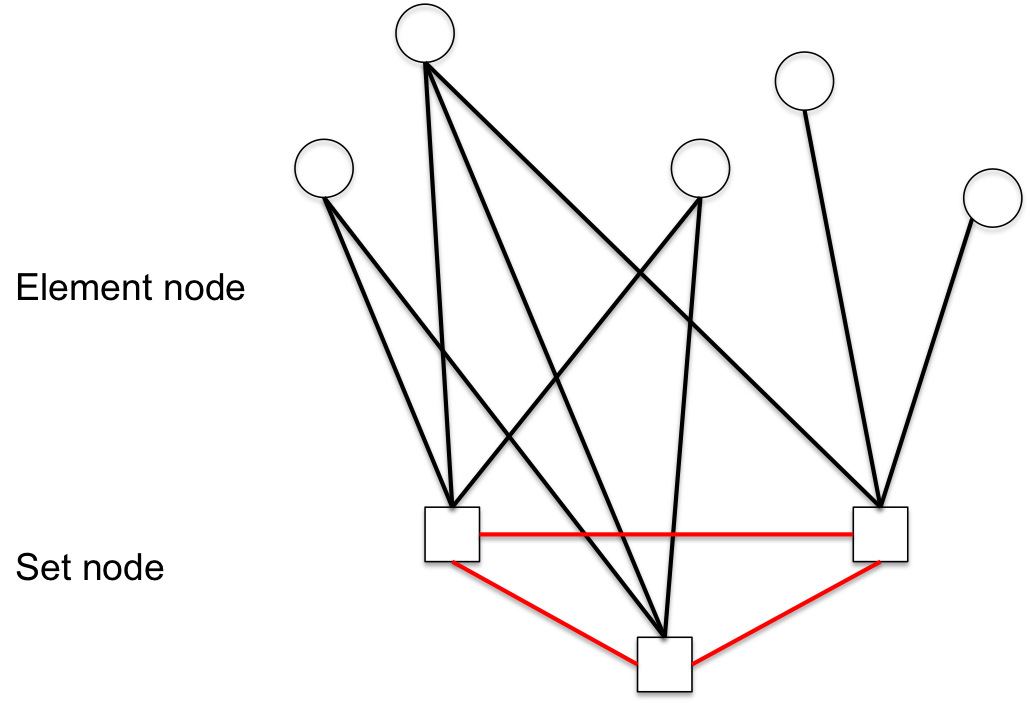
\includegraphics[width=0.6\textwidth]{./setcover.png}
\caption{集合覆盖-距离}
\label{fig:setcover}
\end{figure}


假如我们能在多项式时间内求解原问题。如果存在$L^*$,则取$L^*$对应集合的结点(如果对应元素,替换成任意一个包含它的集合),这样我们就找到了$U$的一个覆盖。如果$L^*$不存在,则集合覆盖也不存在。因此,我们要求解的判定问题是一个NP完全问题。故优化问题是一个NP-Hard问题。不存在已知的多项式时间解。
\end{proof}


\subsection{子模性及近似求解}
前文已经证明最优化$Q(L)$是一个NP-Hard问题,但是下面我们将证明其单调性和子模性,并据此得到一个贪心算法(greedy algorithm), 在多项式时间内得到近似解$Q(L')$, 并且保证
\[
	Q(L^*) \ge (1-\frac{1}{e}) Q(L')
\]

\begin{definition}[子模函数]
从幂集$2^\Omega \to R$的一个函数$f$称为子模函数(submodular function),如果对任意$X,Y \subseteq \Omega, X \subseteq Y$,$\forall x \notin Y$, 有$f(X \cup \{x\} ) - f(X) \geq f(Y \cup \{x\} ) - f(Y)$.
\end{definition}

下面我们分别证明$Q(L)$的单调性和子模性。
\begin{proof}[单调性]
令集合$Y=X\cup{x}$。对任意元素$y \in U - X$, 设$sim_K(y, X) = sim_K(y, t), t \in X]$,
那么,
\[
	|\{ {v_j}|sim({v_j},v) \ge sim(y, t), v_j \in X \} | = K	
\]
由于$X \subset Y$,故有
\[
	|\{ {v_j}|sim({v_j},v) \ge sim(y, t), v_j \in Y \} | \ge K	
\]
从而, $sim_K(y, Y) \ge sim_K(y, X)$。由$y$的任意性,得到
\[
	Q(Y) \ge Q(X)
\]
单调性证完。
\end{proof}

\begin{proof}[子模性]
设集合$X \subset Y$, 对任意$x \in U - Y$, 设$X' = X\cup{x}, Y' = Y\cup{y}$。
对任意$y \in U$, 由单调性有
\[
	sim(y, Y') \ge sim(y, X') \ge sim(y, X) \\
	sim(y, Y') \ge sim(y, Y) \ge sim(y, X) 
\]

对于新加入的元素$x$, 有
\begin{align*}
	sim(y, X') = & \max\{ sim(y, x), sim(y,X) \} \\
	sim(y, Y') = & \max\{ sim(y, x), sim(y,Y) \} \\
\end{align*}

于是
\begin{align*}
	sim(y, Y') - sim(y, Y) = & \max \{ sim(y, x) - sim(y, Y), 0\} \\
						\le & \max \{ sim(y, x) - sim(y, X), 0 \} \\
						= & \max \{ sim(y, x), sim(y, X) \} - sim(y, X) \\
						= & sim(y, X') - sim(y, X)						
\end{align*}
由$y$的任意性,子模性得证。
\end{proof}

\begin{theorem}
对于一个单调增的子模函数$Q$,从空集$L_0$开始,使用贪心策略进行迭代,即第$k$次迭代选取元素$v_k$,使得
\[
	v_k = \mathop {\arg \max }\limits_{v_k \notin L_{k-1} } Q(L_{k-1}\cup \{v_k\}) 
\]
\[
	L_k = L_{k-1} \cup \{ v_k \} 
\]
那么$K$次迭代之后, 对任意$L, |L| \le K$,有
\[
	Q(L_k) \ge (1-\frac{1}{e}) Q(L'),
\]
\end{theorem}

这直接给我们了一个保证下界的贪心算法。
\begin{algorithm}
  \caption{maximize Q(L)}
  \KwIn{Unisersal set $U$, target size $K$ and similarity measure $sim()$}
  \KwOut{${L^*} = \mathop {\arg \max }\limits_{L,|L| = K, L \subseteq U} Q(L)$ }
  $L_0 = \emptyset$\;
  \For{$k=1;k \le K;k += 1$}
  {

  }
  return $con(r_i)$\;
\end{algorithm}

\section{模型选择}
我们的标注集选择和KNN有密切的联系,KNN在我们的数据中可能表现更好,但是我们也会尝试其他的分类模型,如支持向量机,随机森林等。

\section{实验结果与错误分析}
为了检验我们标注和分类的效果,我们从短语候选集中随机抽取了5000个短语作为Ground Truth进行测试。

图\ref{fig:testing_vs_random}是我们分别使用随机抽样(Random)和最大化$Q(L)$(MaxSim)的方法选取500、1000、2000个标注样本时,5-NN分类器在测试集上的表现。对于随机抽样,我们进行5次试验取平均值,并在图中标注了最大和最小值。

\begin{figure}[h!]
  \centering
  \begin{subfigure}{0.4\textwidth}
    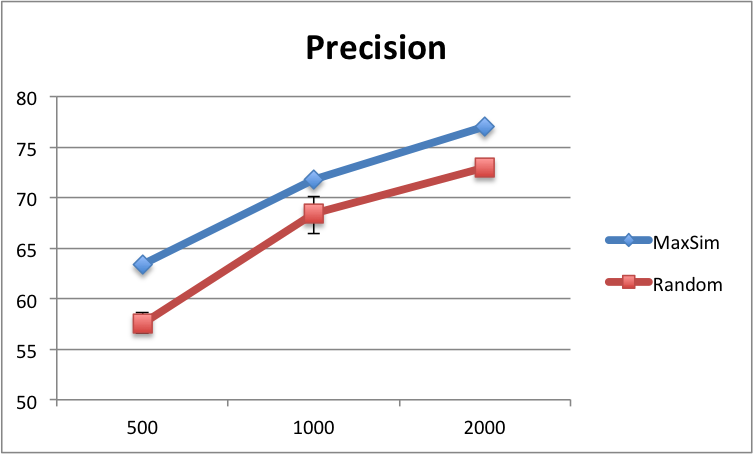
\includegraphics[width=\textwidth]{label_precision.png}
    \caption{Precision}
  \end{subfigure}
  \hspace{2em}%
  \begin{subfigure}{0.4\textwidth}
    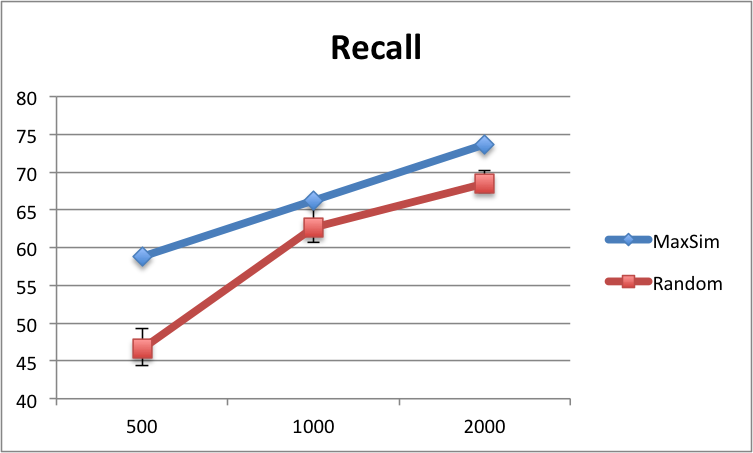
\includegraphics[width=\textwidth]{label_recall.png}
    \caption{Recall}
  \end{subfigure}
  \hspace{2em}
  \begin{subfigure}{0.4\textwidth}
  	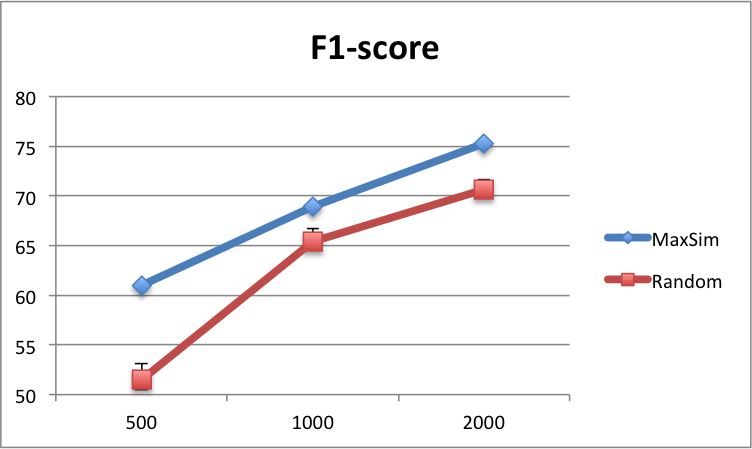
\includegraphics[width=\textwidth]{label_f1.png}
  	\caption{F1-score}
  \end{subfigure}
  \caption{实验结果}
  \label{fig:testing_vs_random}
\end{figure}
从图\ref{fig:testing_vs_random}中可以看出,我们提出了训练集选取方案,在Recall和Precision方面,都稳定的高于随机随机抽样,尤其是在标注量较小时,MaxSim选取的标注集在Recall方面的优势更加明显。

同时我们测试了其他分类模型在两种标注集选取方法下的性能。

可以看出除了KNN以外,SVM,随机森林等分类器在MaxSim上的性能都超过了随机方法。同时,SVM和KNN的总体表现(F1-score)上相差不多,Precision较高而Recall较低,在实际系统中,我们希望提供更加精确的结果,因此,我们最终采用SVM作为分类模型。

\section{错误分析和性能优化}
我对分类错误的样本




\chapter{实例抽取与关系挖掘}
\section{目标}
对于一项活动,除了抽象的活动概念以外,还应有相应的属性,如情感状态、时间、地点。为此,我们定义了活动实例(定义\ref{def:instance}。本章的目标在于,输入一条特定微博$m$, 从中抽取活动相关属性,构建活动的实例$a$;并基于实例抽取的结果,进一步构建活动之间的关系。

\section{活动类别抽取}

在第\ref{chp:concept}中,我们已经抽取出一系列抽象的活动概念。在构建活动实例时,我们首先要获取微博$m$对应的活动概念,即活动类别抽取。

类似于第\ref{chp:concept}章的方法,本文首先使用了规则匹配,首先抽取微博中所有的动词短语,并判断是不是对应一个活动概念,这一步只需判断它是否在抽取出的活动概念集合即可。如果不存在,则认为这条微博包含一个活动。这样做的结果精度为74\%,但召回率仅为56\%。对结果的分析发现,大约有11\%的缺失是由于语法结构的复杂性。用户在表述一项活动时,动作和目标有时并不构成一个简单的动宾短语,例如以下情况
\begin{itemize}
\item 宾语可以前置,如``找本书读了一下午'',
\item 加入复杂的修饰成分,如``陪父母看了一场周星驰拍的很有意思的电影''
\item 以主谓、定中等形式出现。如``练了一天的琴''。
\end{itemize}
这些较复杂的情况,通过简单的词法分析和规则匹配是难以处理的。为解决这个问题,本文对句子进行句法分析,将线性文本处理为依存树。句法分析在当前已有许多成熟的分析器,如Stanford Parse\footnote{http://nlp.stanford.edu/software/lex-parser.shtml}和HIT-LTP\footnote{http://www.ltp-cloud.com/}。

Stanford Parser是斯坦福大学自然语言处理组开发的句法分析工具。它主要面向英语语言,也提供中文、德语、阿拉伯语等其他语种的解析,但它的处理结果并不非常直观。最终本文选择哈尔滨工业大学开源的语言技术平台(Language Technology Platform, LTP)\cite{che2010ltp}作为句法分析工具。LTP提供分词、词性标注、命名实体识别、依存句法分析、语义角色标注等功能,提供自然语言处理的集成解决方案。LTP接收原始文本作为输入,结果以XML的形式给出,对每个词,给出其依赖词和依赖关系,依赖关系包括主谓(SBV),动宾(VOB), 定中(ATT),并列(COO)等。图\ref{fig:ltp_demo}是LTP进行句法分析的结果,它正确分析出``看''和``电影''的动宾关系。

\begin{figure}[!h]
\centering
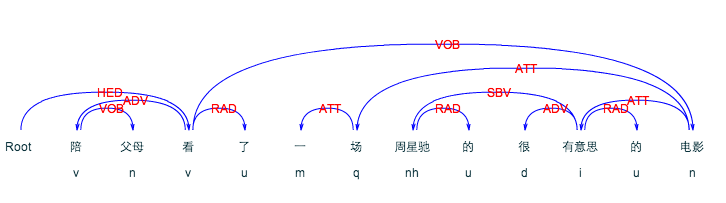
\includegraphics[width=0.9\textwidth]{ltpdemo1.png}
\caption{LTP句法分析示例}
\label{fig:ltp_demo}
\end{figure}

通过LTP进行句法分析,得到词语之间的依赖关系,进一步抽出动词短语,判断是否是一个活动概念,结果如表\ref{table:cat_extraction}。

\begin{table}
\centering
\begin{tabular}{|c|c|c|c|}
\hline
& Precision & Recall & F1 score \\
\hline
Result & 73.2\% & 68.4 \% & 0.707 \\ 
\hline
\end{tabular}
\caption{活动类别抽取实验结果}
\label{table:cat_extraction}
\end{table}

除精度、召回率以外,处理速度也是一个关键的问题。将整条微博作为LTP的输入,处理速度非常慢,分析工作的复杂度随文本长度指数增长。为提高速度,首先将文本分割为多个短句,再进行分析,就可以达到较快的速度。由于不同微博的分析工作是独立的,为了进一步提高处理能力,可以使用多线程、多机进行并发。图\ref{fig:parse_speed}中比较了不同处理策略,分析1000条微博的速度。

\begin{figure}[!h]
\centering
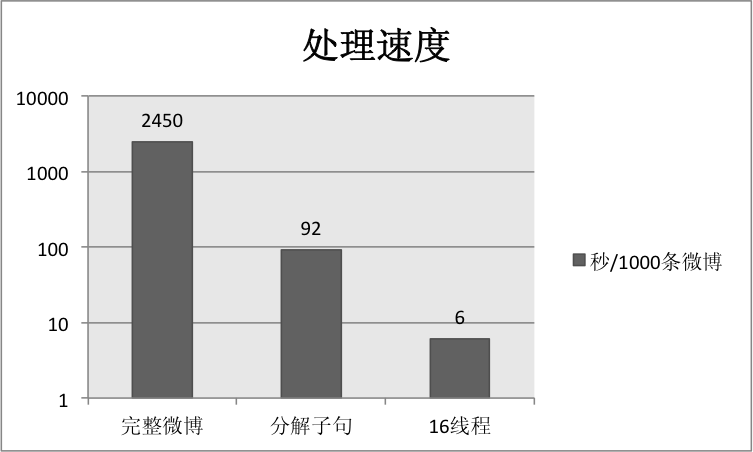
\includegraphics[width=0.7\textwidth]{speed.png}
\caption{分析速度}
\label{fig:parse_speed}
\end{figure}

本文方法的不足在于,没有考虑特定命名实体与活动类别的关系。如,``下午去看了阿凡达''这类微博。``阿凡达''是一部电影的名称,因此这条微博应对应``看电影''这个活动类别,但本文的方法无法正确抽取这类活动。类似的情况如餐馆、电视剧、特定的地名等等。在下一步工作中,可以引入外部的知识库,以建立命名实体与活动的联系。

\section{情感极性分析}
在活动抽取中,如果微博中包含用户参与的一项活动,我们希望了解用户参与这项活动时的心情状态如何,帮助我们发现活动本身是正面还是负面,这样帮助推荐系统进行选择。因此,需要获取微博的情感极性。

\subsection{方法概述}
本文的工作中,对微博进行三分类,正面(positive),中性(neutral)和负面(negative)。

我们对非监督和监督学习均进行了尝试。在非监督的方法中,我们从知网(Hownet)等途径获取了中文的情感词典,共有4986个积极词汇和4818个消极词汇,包含动词、形容词和名词。对每一条微博,我们首先计算计算其中积极、消极词汇的数量$n_{pos}$和$n_{neg}$,若其差值$|n_{pos}-n_{neg}|<\theta$,则认为微博是中性的,否则判别为词数多的类别。但这样简单的非监督方法只能达到55\%的正确率(注意到这是三分类问题,这个结果还是比随机分类(33\%)和全部判为最多的类别(45\%)要好)。为此,我们使用监督学习的方法,使用以下特征训练分类器

\begin{enumerate}
\item Bigrams和Unigrams的频度。使用bigram的原因是,情感词之前常常会带有修饰性的前缀,如``不'',``非常'',有时会加强或者逆转情感词的极性。因此对于较频繁出现的模式,是哟高bigram作为特征。
\item 正面词、负面词出现的频度。这可以根据情感词典得到。
\item 表情符号。用户在发布微博时,常常会加入一些表情,如``高兴'',``愤怒'',有时用户选择表情并不关心这个表情具体的含义是什么,但是也可以体现出用户当时的心理状态。
\end{enumerate}
同时,为了加快训练速度和减少噪声,我们将过于稀疏,即出现次数少于一个下界的特征滤除。

\subsection{实验结果与分析}
我们标注了20829条包含活动信息的微博,根据其情感极性标注为5级,-2为很负面,-1为一般负面,0为中性,1为一般积极,2为很积极,其中分级-2、-1为负面,+1,+2为中性,0为中性。为了避免不同人倾向性的不同,每条微博会有至少两个人标注,如果出现分歧,由实验者最终决定类别。在数据中,共有9462条为中性,6566条为正面,4787条为负面。在此数据上进行交叉验证。

我们首先检验不同特征的选取对分类精度的影响,如图\ref{fig:sentiment_feature}。可以看到,我们选取的特征,对于分类结果都有明显的提升,其中情感词词典的作用最为明显。
\begin{figure}[!h]
\centering
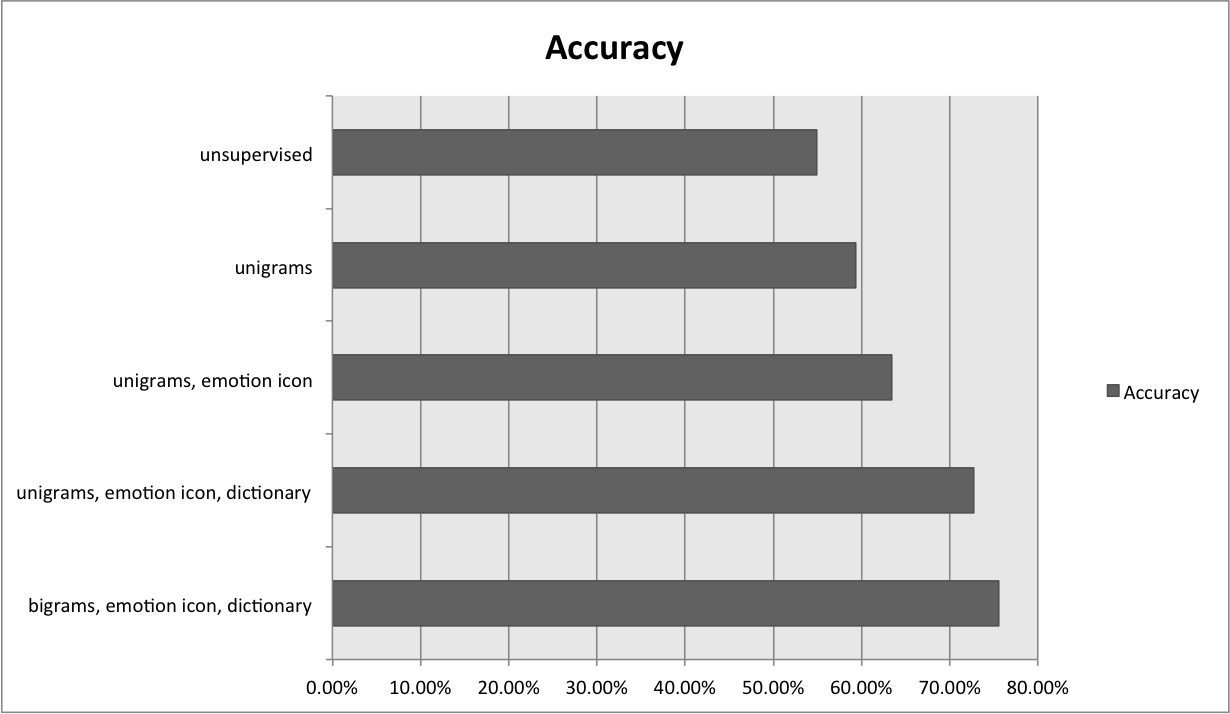
\includegraphics[width=0.9\textwidth]{sentiment_feature.png}
\caption{特征选择}
\label{fig:sentiment_feature}
\end{figure}

本文继续尝试了不同的分类模型,包括
\begin{itemize}
\item 朴素贝叶斯
\item 以决策树为基础的AdaBoost
\item 随机森林
\item 线性核SVM
\end{itemize}
测试结果如图\ref{fig:sentiment_model}。线性核SVM表现最好,但朴素贝叶斯也有比较好的性能,与\cite{pang2002thumbs}中的结果一致。

\begin{figure}[!h]
\centering
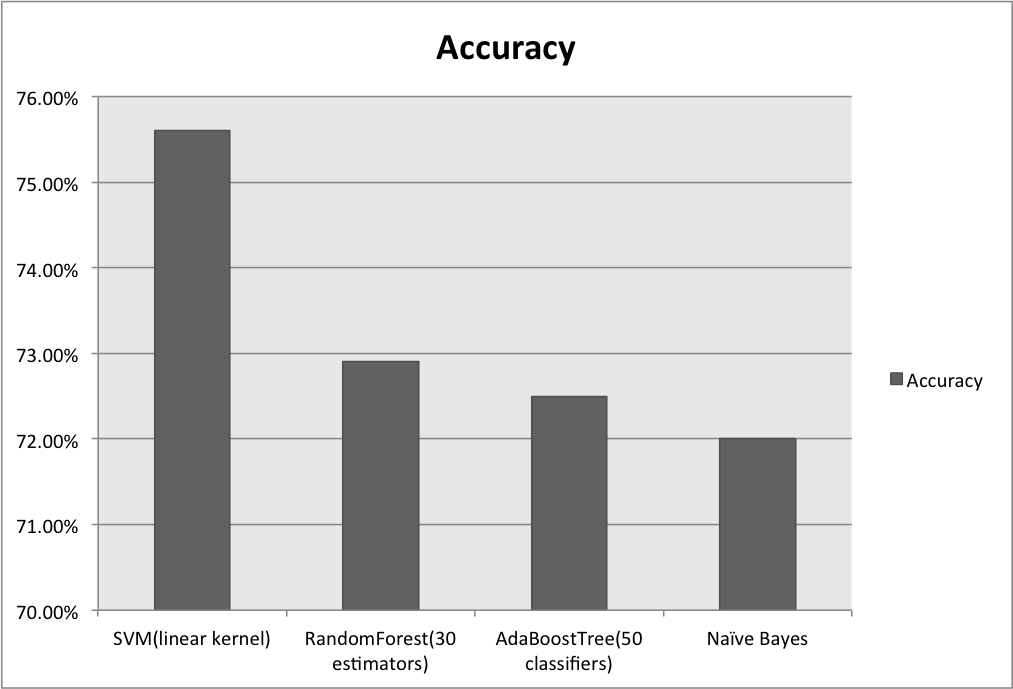
\includegraphics[width=0.8\textwidth]{sentiment_model.png}
\caption{模型选择}
\label{fig:sentiment_model}
\end{figure}

最终达到的75\%的分类精度从数值上看并不是很高,但情感极性的判断有很强的主观性,正面负面和中性并没有很明显的界限。根据之前的研究,人类对情感的判断也只能在79\%的情况下达成一致,因此,一个准确率70\%以上的系统在实际中是可用的。

\subsection{进一步工作}
文档级的情感分类做出了一个假设,即用户在一条微博中只提到一项活动,或者提到多项活动但情感极性是相同的,这在社交媒体短文本的限制下是合理的,在我们的统计中,只有3\%的微博描述多个活动,并且带有相反的情感倾向。但这在实际中并不总是成立。同时,即使同为负面情感,用户的具体情感也可能非常不同,如``疲倦''、``伤心''、``生气''三者代表的情感完全不同,无法用简单的极性表达。Ekman\cite{ekman1992argument}将人类情感分为6中基本情感,``高兴(Happy)'',``激动(Excited)'',``温和(Tender)'',``惊吓(Scared)'',``悲伤(Sad)'',``生气(Angry)''。进一步可以考虑情感的多分类问题。

第二点是,一个活动中会有不同的子方面,如旅游,用户可能会对天气、交通、饮食、住宿等方面分别表达情感。这种基于方面的细粒度的观点挖掘在商品评论中有比较多的研究,下一步工作中会加以考虑。

\section{地点、时间抽取}
新浪微博的数据,可以分为两类
\begin{enumerate}
\item 带有地理信息。通过移动终端发布微博,并开启定位服务,在微博元信息中会包含微博发表时的地理位置,包含经纬度;有些微博还包含对应兴趣点(POI, point of interest)的信息。
\item 普通微博。仅带有发布时间,无法通过元信息直接获取地点。
\end{enumerate}

对于第一类带地理信息的微博,我们可以通过经纬度,直接获取到地点。我们与搜狐合作,得到的国内主要城市的兴趣点数据,来辅助我们的地点抽取。POI数据中包含位置,类型,名称等信息,样例如表\ref{table:poi_sample}。通过经纬度在兴趣点数据中寻找最近的兴趣点,即可获取活动发生的地点,包括城市,地址,POI类型。这些微博占所有微博的16\%,但总数很大,共有620万条左右,对于我们挖掘活动信息已经比较充分了。

\begin{table}[htbp]
\centering
\begin{tabular}{|c|c|}
\hline
{\heiti Attribute} & {\heiti Value} \\
\hline
Name & 北京密云东方商贸大厦 \\
\hline
Address & 北京市密云县新东路40 \\   
\hline
Contact & 010-69043424    \\
\hline
Type & 购物场所        \\
\hline
Category & 一般商场      \\  
\hline
Province & 北京市  \\
\hline
City & 北京市  \\
\hline
District & 密云县 \\  
\hline
Longtitude &13008155.004543  \\
\hline
Latitude & 4892797.007317 \\
\hline
\end{tabular}
\caption{POI样例}
\label{table:poi_sample}
\end{table}

对于第二类微博,我们通过分析文本获取地点信息,这类信息抽取任务可以使用CRF来完成,为了减少标注所需的工作量,我们使用了自监督的方法。可从微博中直接抽取到地点的微博,我们从文本中定位地点的位置进行标注,作为正例训练标注模型。地点信息通常带有明显的上下文特征,可以利用这些信息,对地点进行分类。我们使用以下特征进行分类:
\begin{itemize}
\item 词本身$w_i$,对于常见地点、城市,如``超市''、``北京'',词本身可以提供有效的特征。
\item 词性。地点通常为名词,并且在ICTCLAS的工具中,对于常见地点词,会标记为地点,可以加以利用。
\item 前一个词$w_{i-1}$。我们统计地点词之前一个词的词频,频度最高的词有:在、去、抵达、到达、来、来到等。这些标志词,对地点识别有很大帮助。
\end{itemize}

我们标注了2000条微博中进行测试,结果如表\ref{table:place_extraction}。表\ref{table:place_extraction_sample}是对一些微博进行地点抽取的样例。

\begin{table}[!h]
\centering
\begin{tabular}{|c|c|c|c|}
\hline
& Precision & Recall & F1 score \\
\hline
Result & 62.6\% & 81.4\% & 0.717 \\
\hline
\end{tabular}
\caption{地点抽取实验结果}
\label{table:place_extraction}
\end{table}

\begin{table}[h!]
\centering
\begin{tabular}{|c|c|}
\hline
{\heiti 微博} & {\heiti 抽取结果} \\
\hline 
打车去高铁站 & 高铁站 \\
\hline
奔波一天,终于回上海了 & 上海 \\
\hline
在文华园吃的很nice & 文华 \\
\hline
凌晨五点,寒冷的北京 & 北京 \\
\hline
在长城上跳骑马舞最好玩了 & 长城 \\
\hline
见过人海吗?快来乌镇! & 乌镇 \\
\hline 
我在这里 & 这里 \\
\hline
兰州军区那么多丰田越野车 & 兰州 \\
\hline
就算一车切糕一万元。水果不值钱嘛,去超市看看 & 超市 \\
\hline
在新疆叶城时,天黑去维吾尔族聚居区吃的宵夜。 & 新疆 \\
\hline
\end{tabular}
\caption{地点抽取结果样例}
\label{table:place_extraction_sample}
\end{table}

\section{序列关系挖掘}
知识库系统还需要构建概念之间的关系。与通常的知识库系统一般建模概念之间的上下位关系不同,本文关注活动间的序列关系(follow-up relation),即用户在参加一项活动后,通常进行的下一项活动是什么。这一点有助于帮助我们对用户行为进行建模,进行活动的推荐。

通过之前的工作,我们已经在微博中抽取出大量活动的实例,序列关系的抽取可以在这个基础上进行。序列关系的强弱包含两个方面
\begin{enumerate}
\item 用户进行活动$c_i$后,在时间窗口$T$内,进行活动$c_j$的概率
\item 用户进行活动$c_i$和$c_j$之间的期望时间
\end{enumerate}
这两个方面缺一不可。由于用户行为的复杂性,第一项可以对噪声进行抑制,避免个别用户随机行为的影响,使挖掘出的活动有较高的置信度;第二项表示两项活动间隔的时间越短,它们的序列关系越密切。基于这两个考虑,我们对问题定义如下:

\begin{problem}[序列关系挖掘]
给出
\begin{itemize}
\item 活动概念集合$C={c_i},i=1,2,\ldots,N^c$,$N^c$为活动概念的数量。
\item 用户集合$U=\{u_i\},i=1,2,\ldots,N^u$,$N^u$为用户数量
\item 活动实例集合$A = {A_i}$。对每个用户$u_i$,有其参加活动实例的集合$A_i = \{a_{ij}\}, j=1,2,\ldots,N_i^a$,$N_i^a$是用户$u_i$在给定微博语料中参与活动实例的个数,每个活动实例$a_{ij}$是活动概念、时间、地点、情感极性的四元组,即$(c,t,p,s)$。
\end{itemize}
求在给定时间窗口$T$内,
\begin{enumerate}
\item 用户进行活动概念$c_i$后进行活动$c_j$的概率$P(c_i|c_j,T)$
\item 在$P(c_i|c_j,T)>\lambda$的条件下,$E(t_{c_j} - t_{c_i})$
\end{enumerate}
\end{problem}

根据问题的定义,可以得到算法如下:

\begin{algorithm}
  \caption{序列关系挖掘}
  \KwIn{活动实例集合$I$, 用户集合$U$, 每个用户$u_i$的活动实例集合$A_i$, 活动概念集合$C$, 阈值$\lambda$, 时间窗口$W$}
  \KwOut{对每个活动概念$c_i\in C$, 随后可能发生活动的序列$seq_i$}
  \ForEach{$A_i \in A$}{
	 \ForEach{$a_{ij} \in A_i$}{
	  	\ForEach{$a_{ik} \in A_i, t_{ij}<t_{ik}<t_{ij}+W$}{
	  		$seq\_occur(c_{ij}, c_{ik}) += 1$\;
	  		$past\_time(c_{ij}, c_{ik}) += t_{ik}-t_{ij}$\;
	  	}
	 }
  }

  \ForEach{$c_i \in C$}{
		$follow_{c_i} = \{c_j | \text{seq-occur}(c_i, c_j)>\lambda \}$\;
  		sort $follow_{c_i}$ by past\_time($c_{ij}, c_{ik}$)/seq-occur($c_{ij}, c_{ik}$)\;
  		$seq_i$ = $follow_{c_i}$\;
  }
  return $\{seq_i\}$
\end{algorithm}

在我们的系统中,时间窗口取6小时。为了查询时的快速响应,本文对所有活动离线进行计算,对每项活动,记录序列关系最强的10项活动。

\section{本章小结}
本章关注活动实例中属性的抽取,包含类别、地点、时间、情感极性等。我们使用句法分析器HIT-LTP提高的活动抽取的召回率。在情感分类中,通过情感词词典,本文训练了分类模型,取得了较好的分类效果。在地点抽取中,我们借助已有的地理信息和POI数据,使用了自监督的学习方法,避免了繁重的手动标注。最后基于实例抽取的结果,我们分析了活动间的序列关系。



\chapter{ActivityNet系统设计}

\section{设计目标}
通过之前的工作,本文从社交媒体中抽取了活动概念、地点、情感等属性,并挖掘了活动间的相关性和序列信息。基于这些工作,本文构建了一个可视化系统ActivityNet。系统希望实现以下目标:
\begin{itemize}
\item 高效的活动检索
\item 良好的可视化界面
\item 提供用户反馈机制,纠正错误分类
\end{itemize}

\section{底层架构}
考虑到系统将来的可扩展性,我们选择SAE作为系统底层架构。SAE全称为Social Analytic Engine,即社交网络分析引擎,是清华大学计算机系KEG研究组开发的一套社交网络分析平台,架构图见图\ref{fig:sae_arch},提供了以下功能:
\begin{enumerate}
\item 存储和快速检索极大规模社交网络的数据
\item 提供最新的社交网络分析算法和机器学习算法,如话题模型(Topic Model), 影响力最大化模型(Influence Maximization)等
\item 提供通用的网络分析引擎和机器学习引擎.
\end{enumerate}

\begin{figure}[!h]
\centering
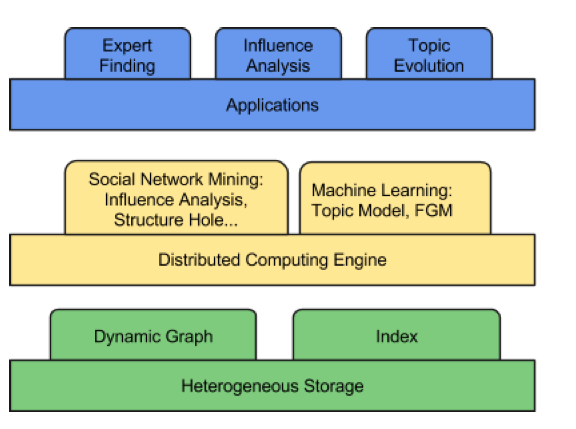
\includegraphics[width=0.7\textwidth]{sae.png}
\caption{SAE基本结构}
\label{fig:sae_arch}
\end{figure}

在ActivityNet中,我们主要用到SAE的存储和索引机制。由于SAE主要用于处理社交网络数据,因此图是SAE主要的存储模型。本文将活动以及之间的关系抽象为图结构进行存储。为了检索的高效,对所有活动名称建立了索引。同时,由于相似活动搜索是基于语义相似度的,本文也对词向量使用KD-Tree进行索引。

\section{功能实现}
ActivityNet以Web站点的形式提供服务,基于成熟的前端框架$Twitter Bootstrap$,简化了开发工作。下面我们以查询``吃烤鸭''为例,介绍系统中各个功能。

\subsection{首页设计}
ActivityNet的首页如图\ref{fig:frontpage}。

\begin{figure}[!h]
\centering
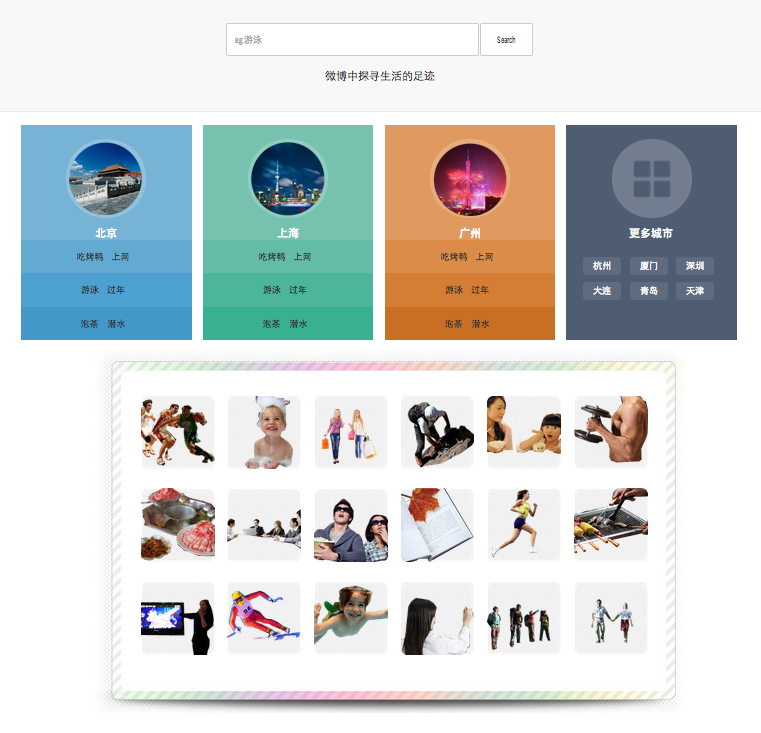
\includegraphics[width=\textwidth]{frontpage.png}
\caption{Activity首页设计}
\label{fig:frontpage}
\end{figure}

首页提供以下功能
\begin{enumerate}
\item 活动搜索。用户可以自行输入自己希望查询的活动
\item 城市热门活动推荐。我们计算出北京、上海、广州的热门活动,在首页进行推荐。
\item 全网热门活动。基于活动实例抽取结果,我们选择了18个最热门的活动,在首页底部呈现。活动对应的图片是以活动本身为关键词构建GET请求,在百度图片搜索抓取第一张图。自动抓取的个别活动图片不很理想。我们在自动抓取图片后,人工进行一些调整。
\end{enumerate}

\subsection{活动搜索}
用户输入一个查询后,可以进入此活动查询结果的二级页面。在此,输入``吃烤鸭'',查询结果如图\ref{fig:query_kaoya}

\begin{figure}[h]
\centering
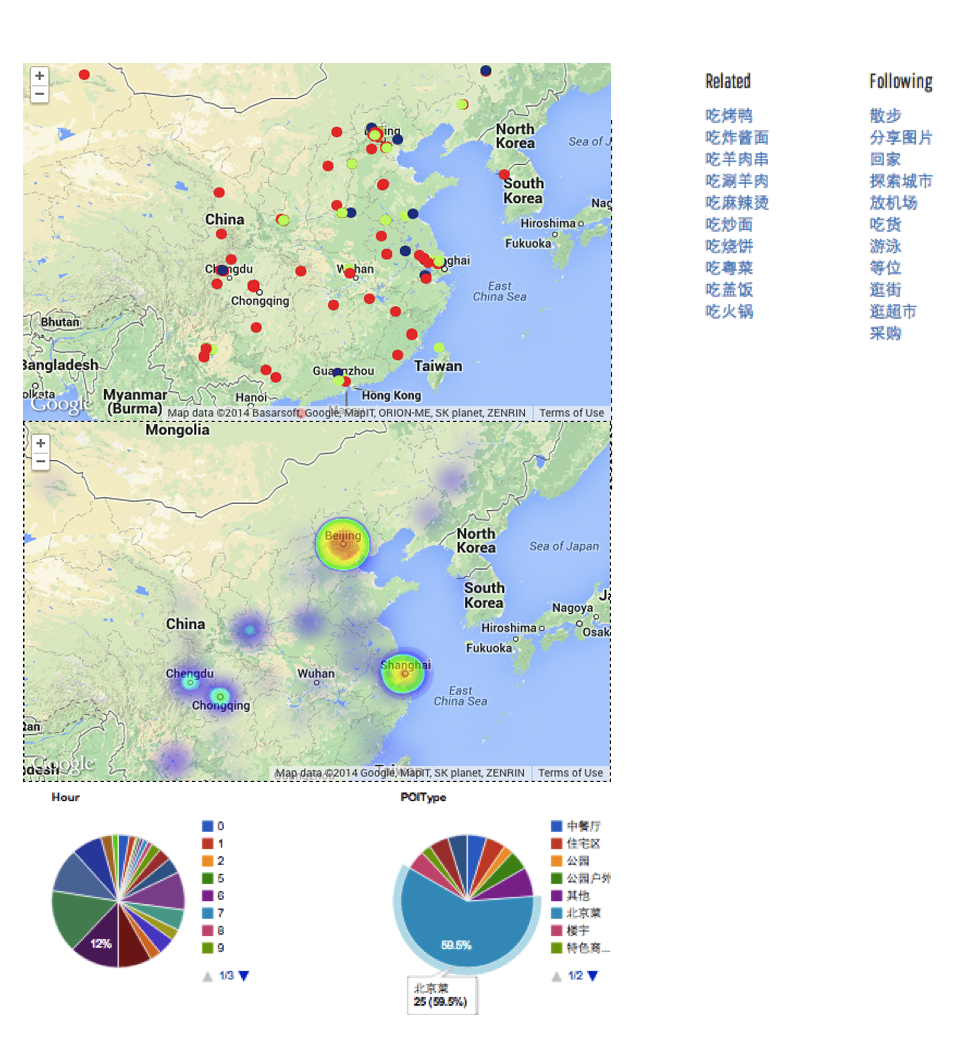
\includegraphics[width=\textwidth]{kaoya_new.png}
\caption{查询结果}
\label{fig:query_kaoya}
\end{figure}

在页面右侧,我们列出了和查询相关的前10个活动,以相关性排序;其次,利用序列关系抽取的结果,我们列出了此活动经常发生的后续活动。烤鸭是北京的特色菜品,``相关活动''中,我们列出的``炸酱面'',``涮羊肉'',``麻辣烫''也都是北京的特色菜。在序列关系中,ActivityNet提供了``散步'',``回家'',``游泳'',``探索城市'',``逛街'',``逛超市''等活动,是比较合理的。由于概念的抽取难以做到完全的精准,ActivityNet的结果中有一些噪声,为此,我们提供用户反馈机制。如果用户发现返回的结果不是活动,鼠标移上之后会呈现``$\times$''按钮,点击后会向系统报告错误。

\subsection{地点、情感、时间分布}
基于地点抽取和情感分类的结果,本文利用Google Map API将地理分布和情感分布可视化。上图是用户在参加活动是情感状态的分布,一个圆点表示一个活动实例,红色为正面情感,蓝色为负面情感,绿色为中性。下图是这项活动的在不同地域的分布情况,以不同颜色的弥散圆表示,红色的强度表示和这项活动相关的活动相关的微博数目。可以看到,``吃烤鸭''这项活动,在北京最为流行;在上海、成都、重庆等地也有着较多的分布。

进一步分析了这项活动发生的POI的类型。从POIType的饼状图中可以看到,``吃烤鸭''最常发生在``北京菜''这类POI中,其次还有为``中餐厅''。而在时间分布中,``吃烤鸭''最常发生的时间为6点。

\section{本章小结}
本章从底层架构到界面设计介绍了基于活动信息挖掘的可视化系统ActivityNet。ActivityNet基于SAE(Social Analytic Engined)实现了高效的存储和检索功能,并利用gchart和Google Map API实现信息可视化,实现了较好的用户体验。由于方法的局限,ActivityNet呈现的结果有一些噪声,系统中提供了用户反馈机制,使得不正确的结果可以及时更正。



\chapter{结论和进一步工作}

\section{工作总结}

随着社交网络的蓬勃发展,人们的线下生活越来越多地反映到社交媒体发布的信息中。通过对社交媒体中用户表达的日常活动进行发掘,能够发现关于活动的许多知识,诸如地域偏好,时间分布,活动之间的概念联系。同时,我们也能够了解到用户的个人喜好,行为模式,对用户进行个性化推荐。例如,用户来到一个新的城市,可以根据他在社交网络中的历史信息以及其他用户在这个城市参与的活动,像他推荐感兴趣的活动项目。

本文对相关研究进行挖掘,确定了三个研究内容:(1)如果精确地从社交媒体中抽取出日常活动的概念表示?(2)针对用户发布的信息,如何抽取出相关活动及相关属性,如地点、时间、情感?(3)如何构建活动之间的关系层次?对于第一个问题,我将抽取问题转换为分类问题,使用神经网络语言模型word2vec获得个短语的语义向量表示,并训练分类模型,取得了较好的分类精度。第二个问题中,我借助哈工大LTP工具,并利用微博自身元信息和POI数据,构建出活动的实例。第三个问题,我参考\cite{wang2013phrase}中提出的框架,构建了活动的层次关系,并对微博时间序列进行统计,得到活动序列关系。

基于以上三点研究,我构建了基于SAE(social analytic engine)的演示系统,对于用户的查询,将活动相关的知识可视化。

\section{局限和进一步工作}

本体学习已经有很长的历史,但在社交媒体中挖掘活动相关知识很少有前人的工作。本文在这一课题上进行尝试性的研究,并构建了初步的原型系统,但由于时间和能力所限,还有不少局限性。在将来,需要在以下方面进行改进:
\begin{enumerate}
	\item 考虑用户在社交网络中的互动关系。用户的好友和网络结构可以提供关于用户的很多信息。例如,用户在进行活动时提到了他的好友,可能隐含其好友也在参与了这项活动,而在当前的工作中,用户作为一个个体存在,并没有考虑到用户间的互动。
	\item 对活动关系的建模比较粗糙。活动之间的关系式多样的,并不能简单的用上下位、follow-up来概括。我们需要构建活动知识的图,而不是简单的层次。
	\item 本文现阶段的工作,仅在社交媒体的数据进行挖掘。如果能现有的知识库,如地点、人物、书籍等结合,能对活动抽取和关系建模有很大的帮助。
\end{enumerate}

希望本文的研究可以继续发展,成为成熟的系统,为用户提供服务。
\chapter{活动关系抽取及知识发现}
\section{构建活动层次}
如何从一系列概念中挖掘出层次关系,目前有一些工作,例如KDD2013年的一篇文章\ref{wang2013phrase},是在科技文献中构建研究领域的层次关系,本文在其基础上进行扩充和修改,以适应活动层次挖掘的任务。

\subsection{算法概述}



\section{序列关系挖掘}
\section{时间、地域分布挖掘}


%%% 其它部分
\backmatter

% 本科生要这几个索引,研究生不要。选择性留下。
\makeatletter
\ifthu@bachelor
  % 插图索引
  \listoffigures
  % 表格索引
  \listoftables
  % 公式索引
  %\listofequations
\fi
\makeatother


% 参考文献
\bibliographystyle{thubib}
\bibliography{ref/refs}

% 致谢
%%% Local Variables:
%%% mode: latex
%%% TeX-master: "../main"
%%% End:

\begin{ack}
  衷心感谢导师唐杰副教授的精心指导。他的言传身教将使我终生受益。

  感谢陈麒聪、曹烨、杨洋同学,他们参与了我的毕业设计的工程中,并给了我很多帮助。
  在美国南加州大学进行暑期研修期间,承蒙Ugur Demiryurek教授热心指导与帮助,不
  胜感激。感谢IBM中国研究院的蔡柯柯研究员,和她的交流给了我许多灵感和想法,让我获益良多。
  
  感谢陈朝松、仓馥芝和张越辅导员,他们的帮助,让我克服了大学中生活、学业遇到的种种困难。还要感谢金昊衠学长,他在超级计算机竞赛期间,给予了我非常多的帮助。
\end{ack}


% 附录
\begin{appendix}
%%% Local Variables: 
%%% mode: latex
%%% TeX-master: "../main"
%%% End: 

\chapter{外文资料的调研阅读报告}
\label{cha:engorg}

Online social networks, such as Facebook, Twitter, Weibo and Renren, have achieved great success in the past years. Now Facebook has over 1 billion users and Sina Weibo has about 59 million users. It's reported that people in US are spending their 16\% online time on Facebook, even more than Google (10\%). With the rapid growth of online social networks, information is produced at an amazing speed. More than 500 million tweets are sent everyday on average. people share their opinions about various events from the Olympics to commercial promotions. Each event consists of several aspects and people's interests and opinions are changing over time. Take the Olympics for example. The opening ceremony is mostly talked about in the first few days. Then with the event going on, different sport matches and athletes are talked about. When an athelete won a pedal, people will cheer for him. However, severval days later, he made a blunder and lost, people's opinion changed. Faced with the information overwhelming, we need a automatic way to track the event process and people's opinon. Given an event, we want to know, 1. What aspects does people interested in 2. How does people's interest and opinions evolve over time and 3. Who are the most influcial users in the discussion of the topic. And finally a flow chart visualization is helpful to demostrate the evolution process of the opinion.

Several classical research areas in data mining are closely related to the problem, such as opinion mining, topic modeling, event detection and tracking. 

\section {Opinion Mining}
Opinion mining aims to find out people's opinion about an {\em entity} from corpus like product reviews or blogs. An entity can be a product, service, event, topic, anything that can be evaluated. An entity can be represented as a combination of different aspects (or features). For example, for an mobile phone (entity), screen, battery, memory are three aspects. Given a collection of documents $D$, the objective of opinion definition is, opinion mining aims to extract entities, aspects, associated opinions and analyse their sentiment orientations. To get a high-level perspective of the whole corpus, an addition summary step is optional.

Aspect extraction is a foundametal step in aspected-based opinion mining and is closely related with our task. The first work in aspect extraction is a two-step unsupervised method \cite{hu2004mining}. First, find frequent nouns and noun phrases. Then, find infrequent aspects by using the relationships between aspects and known opinion words. The method base on the intuition that important aspects are talked about frequently and phrases which co-occur with opinions words often are likely to be aspects. Opinion words can be generated in two ways. The dictionary-based approach defines a seed set of opinion words and search their synonyms and antoyms in a dictionary WordNet. However, it fails to capture the characteristic that the same word can express different sentiment orientation in different domains. The corpus-based approach also uses a seet set. But it finds new words by exploiting syntactic or cooccurence patterns in a large corpus\cite{hatzivassiloglou1997predicting}. The aspect extraction and opinion words finding can reinforce each other. New-found opinion words provide hint for identifying new aspects, while new aspects result in more opinion words. So many following researches combine them in a unified framework. 

More unsuperived and supervised algorithms were proposed since then. Supervised methods treat aspect extraction as a classification problem. CRF is used in \cite{jakob2010extracting}. Jin et al. \cite{jin2009opinionminer} used a HMM based sequence tagging method to find entities and opinion words simultaneously. Su et al. \cite{su2008hidden} proposed a clustering-based method to find hidden association of opinion words and aspects. Topic models can also be used in aspect extraction. However, as Titov\cite{titov2008modeling} pointed out, plain LDA is not suitable for aspect extraction because it can't distinguish global topics (like hotels in China, hotels in America) and local topics( aspects of hotels). He proposed a multi-grain LDA (MG-LDA) to solve that problem. MG-LDA models global and local topics at the same time. Another way to solve that problem is to run LDA on sentence level \cite{brody2010unsupervised}. But the two methods mess opinion words and aspects together. Zhao et al, \cite{zhao2010jointly} proposed MaxEnt-LDA to model aspect and aspect-specific opinion words jointly.

To decide the sentiment orientation of an opinion, machine learning classification methods such as SVM and naive Bayesian can be used. However, lexicon-based method can caputure more subtle semantic elements of a opinion\cite{ding2008holistic}. For example, opinion shifters like negation words (not, never, none) and sarcasm, and but-clauses. 

\section {Evolutionary Topic Models}
LDA, first proposed by Blei et al,\cite{blei2003latent} has become the most popular topic modeling tool. In general, LDA is extended in three main directions. 1. Modeling more latent attributes like sentiment, social role, personal preference. 2. Incorporating inter-document relations. For example, relational LDA\cite{chang2009relational} on a citation network and author-topic LDA\cite{rosen2004author} on a author-document network. 3. Build time-aware topic model to model {\em topic evolution} in corpus, which we are most interested in.

The first try to model topic evolution with LDA is by Blei et al\cite{blei2006dynamic}. In their model, time is discretized and topic distributions satisfy Markov attribute. They chain prior $\alpha$ and $\beta$ in LDA with parameters in adjacent time slices using Gaussian distribution. A drawback of discrete-time model is we have to choose a suitable grain of time slices. In continuous dynamic topic model (cDTM) \cite{wang2012continuous}, Brownian motion is used instead of Gaussian distribution. To get rid of the Markov assumption, Wang \cite{wang2006topics} associated a Beta distribution of time with each topic to model topic popularity evolution, but topic distribtuions keep the same over time. Moreover, topic number is fixed over time. Topic birth and death are ignored. For example, at the dawn of artificial intelligence, areas like pattern recognition, natrual language processing are rarely talked about explicitly. However, they're now so important that PR and NLP should be seen as separate topics. So a {\em split} of a topic happens. A non-parametric version of dynamic topic model called Infinite Dynamic Topic Models (iDTM) is given by Ahmed \cite{ahmed2012timeline}. iDTM models each document using a hierarchical dirichlet process.

Visualization is a perfect way to demonstrate the evolution trend of topics. Liu composed several great visualization tools for rendering topic dynamics. TextFlow \cite{cui2011textflow} renders the whole corpus as a multi-branch flow. Each branch is a topic. Different branches can split or join each other, representing topic birth and death. And width of a flow indicates the popularity. It was further developed into a interactive analysing tool \cite{liu2009interactive}.

\section {Event Tracking and Burstiness detection}
The task of Event tracking is about discovering temporal intensities of events in text streams such as weblogs or newswires. Event detection and tracking is closely related with dynamic topic modeling and share methods in common. However, event detection has its own features. First, topic evolution analysis is usually done off-line. We accumulate data over a time window and run algorithms on whole data set. While event detection is executed at the time new data comes, aka {\em on-line}. Second, topic model focuses on topics that are heavily talked about. While event detection emphasizes the {\em burstiness} more. A new event may not be talked about intensively now, but its occurence rises rapidly in a short time. 

Variations of LDA are used in event tracking. AlSumait\cite{alsumait2008line} proposes an on-line version of LDA to track the event. Ha-Thuc et al. proposed a relevance-based topic model for news event tracking\cite{ha2009relevance}.   
However, apart from LDA, many other models can be used. Leskovec et al. \cite{leskovec2009meme} studied a novel problem of meme-tracking. meme is a quoted text which vaires during spreading over the web. They adopted a clustering method to group variants of a meme together and analyisis global and local intensity.

Term burstiness has been extensively researched as a mechanism to address new event detection. Kleinberg \cite{kleinberg2003bursty} used a state machine to model the burtiness and inspired most following work. Lappas et al. \cite{lappas2009burstiness} further explore how burtiness can enhance document searching.



%\bibliographystyle{plain} %
%bibliography{opening.bib}




\end{appendix}

% 个人简历
\begin{resume}

  \resumeitem{个人简历}

  1992 年 1 月 23 日出生于山东省枣庄市。
  
  2010 年 9 月进入清华大学计算机科学与技术系计算机科学与技术专业攻读工学学士学位至今。2010年获新生二等奖学金,2011年获国家奖学金,2012年获清华之友-董氏东方奖学金,2013年获计算机系最高奖钟士模奖学金。另外,于2013年获得中国计算机学会颁发的CCF优秀大学生奖,以及ASC13亚洲大学生超级计算机竞赛冠军,ISC13世界大学生超级计算机竞赛第二名。
  
\end{resume}

\end{document}
